\newif\iflatextwoe
\newif\ifepsf
\newif\ifpsfiginstalled

%
% The following should be set according to whether you have 
%
%    1) latex2e or latex 2.09,
%    2) epsfig,
%    3) psfig installed in your latex.
%
% Peter needs:  true,   true,   irrelevant
% Steph needs:  false,  false,  false
% Terry needs:  false,  false,  true
%
% Therefore...
%
% I have things this way:
%
\latextwoefalse
\epsffalse
\psfiginstalledtrue
%
% Peter, you should have the following 2 lines uncommented:
%
%    \latextwoetrue
%    \epsftrue
%
% Steph, you should have the following 3 lines uncommented:
%
%\latextwoefalse
%\epsffalse
%\psfiginstalledfalse
%


%
% Nothing below here should need to be changed for others to get
% their latex to work on this file.
%

%
% If you add text that depends on latex2e or psfig/epsfig, you can use 
% conditionals to make sure your changes will work for everyone. E.g.,
%
%    \ifepsf
%    \epsfysize=5.5in
%    \epsfbox{figures/preston-curves.ps}
%    \else
%    \psfig{figure=figures/preston-curves.ps}
%    \fi
%
% Specifies a figure in such a way that we can all run latex with 
% no problem.
%
% Of course one way might look better than another and we can decide on
% which to use for the final version later. But for now I just want to
% make it so we can all hack on the text without having to reconfigure a
% bunch of little things every time we get the file.
%
% Terry.
%


\ifepsf
\documentstyle[12pt,epsfig]{article}
\else
\ifpsfiginstalled
\documentstyle[12pt,psfig]{article}
\else
\documentstyle[12pt]{article}
%\input{epsfig.sty}
\input{psfig.tex}
\fi
\fi

\iflatextwoe\else
\newcommand{\emph}{\em}
\fi

\oddsidemargin=0.0751in
\evensidemargin=0.075in
\textwidth=6.5in

\begin{document}
\title{\bf The Ecology of Echo}

\vspace{0.25in}

\author
{
{\bf Terry Jones} \\
Santa Fe Institute \\
1399 Hyde Park Road \\
Santa Fe NM 87501 \\
terry@santafe.edu \\
\and
{\bf Peter T. Hraber} \\
Dept.\ of Biology \\
University of New Mexico \\
Albuquerque NM 87131 \\
pth@santafe.edu \\
\and 
{\bf Stephanie Forrest} \\
Dept.\ of Computer Science \\
University of New Mexico \\
Albuquerque NM 87131 \\
forrest@cs.unm.edu \\
%\and
%{\bf John H. Holland} \\
%Dept.\ of Psychology \\
%University of Michigan \\
%Ann Arbor MI 48103
}

\maketitle

\begin{center}
ABSTRACT GOES HERE.
\end{center}
           \newpage
\section{Introduction}
\label{intro}

Many interesting systems are difficult to analyze and control using
traditional methods.  These include natural ecosystems, immune
systems, cognitive systems, economies and other social organizations,
and arguably, modern computers.  One source of difficulty arises from
nonlinear interactions among system components.  Nonlinearities can
lead to unanticipated emergent behaviors, a phenomenon that has been
well documented and studied in physical, chemical, biological, and
social systems [CITE TAYLOR, ALife II?], as well as in some forms of
computation \cite{Forrest91b}.  Nonlinear systems with interesting
emergent behavior are often referred to as {\em complex systems}.  A
second form of complexity arises when the primitive components of the
system can change their specification, or evolve, over time.  Systems
with this additional property are sometimes called {\em complex
adaptive systems\/}
\cite{Holland95a}.  Here, we will use the term {\em complex adaptive
system\/} (CAS) to refer to a system with the following properties:
\begin{enumerate}
\item A collection of primitive components, called ``agents.''
\item Interactions among agents and between agents and their
  environment.
\item Unanticipated global behaviors that result from the
  interactions.
\item Agents adapt their behavior to other agents and environmental
  constraints.
\item System components and behaviors evolve as a consequence (4).
\end{enumerate}

% There are also all the usual problems of
% verifying that complex simulation code is correct.  

It can be quite difficult to model systems with these properties
analytically.  Useful and predictive mathematical treatments are
difficult, due primarily to the following: nonlinearities (as
discussed above), discreteness, spatial inhomogeneities, and the
changing behavior of the primitive elements of the system.
Discreteness arises, for example, in time (as in the case of
generations in population genetics), state spaces, and internal
variable values, while spatial heterogeneities arise through resource
gradients, nonuniform operating conditions (e.g., different mutation
rates in different parts of the body [cite Kepler and Perelson], or
even random drift.  Both discreteness and spatial heterogeneity can
have a significant effect on system behavior.  For example, Durrett
and Levin \cite{DurrettAndLevin93a} present an elegant description of
how both both properties affect the predictive power of conventional
methods, including ordinary differential equations and
reaction-diffusion systems, on a classical problem in ecology.  As a
consequence, many of the standard approximations for infinite-sized
systems and techniques developed for studying asymptotic behavior of
continuous nonlinear dynamical systems cannot be directly applied to
discrete or spatially heterogeneous systems.  Finally, adaptation is
central in CAS\@.  Because the primitive components of the system can
change over time, different agents may behave according to different
rules at different times.  Individual variants are important and can
determine the overall system trajectory, which precludes modeleing
only their aggregate behavior.  Although the underlying evolutionary
mechanisms themselves can in principle be modeled, as suggested in
\cite{Farmer90}, this is a difficult undertaking, and most such
efforts to date have been notably unsuccessful in describing the
behavior of any particular evolutionary system.
[...this is a difficult undertaking and this level of detail is
usually omitted when modeling complicated systems.  Further, outcomes
of stochastic processes or ``frozen accidents'' can have irreversible
effects on system dynamics \cite{GellMann94,GellMann95}.  Omit rest
of paragraph...PTH] 
For example, analytical models in population genetics typically
describe two-locus systems at equilibrium, often assuming infinite
population sizes, while the cases in which we are interested involve
relatively small populations with richer interactions (i.e., longer
genomes).

An alternative to analytical models of CAS is simulation.  Detailed
simulations are also problematic, because it is often impossible to get
all of the details correct.  Consider, for example, the vertebrate
immune system which has been estimated to express over $10^7$
different receptors simultaneously [STEPH: REFERENCE].  Modeling the
physical chemistry of just one receptor/ligand binding event, even at
an abstract level, requires enormous amounts of computation, and it is
therefore infeasible to model the expressed repertoire of receptors
precisely.  This problem exists for many large complicated systems,
but because nonlinear systems can be highly dependent on seemingly
small details, even a trivial inaccuracy in the model could lead to
wildly erroneous results.  One approach to this problem is to strip
away as much detail as possible, retaining only the essential
interactions.  The goal is then to develop models whose behavior is
robust with respect to the details of the interactions (e.g., avoiding
parameter tweaking to coax a system to produce desired behaviors), and
which produces the broad categories of behaviors in which we are
interested.  An implication of this approach is that such models will
rarely, if ever, be able to make precise quantitative predictions.
The model described in this paper, called Echo, is an example of this
approach, as are many artificial-life models.

Echo is a mechanistic model in the sense that it encodes (as a
computational artifact) a theory about which mechanisms are most
relevant in ecosystems.  In Echo, certain primitive components and
interactions are built in, and when the model is ``run,'' i.e.,
simulated, these mechanisms give rise to various macro-level
properties.  The goal is that the relevant behaviors will arise
spontaneously as a consequence of the primitive mechanisms.  This is
quite a different kind of explanation than simply predicting what will
happen next without representing the underlying mechanisms explicitly.
Of course, prediction is important for models like Echo, but it is
quite a different kind of prediction than that typically associated
with simulations.  In this paper, we use the word ``model'' to
describe the design decisions we have made about which components and
interactions are included and which are not.  This might be confusing
because the model is described in terms of computational structures,
like ``agent,'' ``stack,'' and ``rules.''  Our model is really a
high-level simulation of generic ecological behavior.

%This style of modeling is quite different from the
%differential-equation style of models used most frequently to model
%nonlinear dynamical systems.  In agent-based models, each ``actor''
%and each interaction among actors (i.e., not just each type of
%interaction) is represented (simulated) explicitly.  Individuals are
%capable of quite different kinds of behaviors (the agents in the
%system are heterogeneous).  Agent-based models are discrete in most
%dimensions, typically time, state, and update rules.  As a result,
%these computational models are difficult to analyze.

Echo is related to several earlier CAS models.
Genetic algorithms \cite{Holland92} focus on the evolutionary
component of CAS\@.  They are reasonably well understood and mature,
but ignore several important features, including resource allocation,
heterogeneity, and endogenous fitness.  Classifier systems
\cite{HollandEtAl86} apply genetic algorithms to a cognitive modeling 
framework.  Similarly, Echo extends genetic algorithms to an
ecological setting, adding the concepts of geography (location),
competition for resources, and interactions among individuals
(coevolution).  Echo is intended to capture important generic
properties of ecological systems, and not necessarily to model any
particular ecology in detail.  Echo's contribution to ecological
modeling lies in the fact that evolution is built in as a fundamental
component of the system.  Most existing ecological models 
\cite{May74,Caswell89,DeAngelisAndGross92} do not have such an evolutionary 
component.  Thus, it is difficult to address issues such as flows of
information and resources in many-species assemblages, patterns
of speciation and extinction in ecological communities, and effects
of spatial heterogeneity on population dynamics.

Echo also resembles more recent CAS implementations.  These include Swarm
\cite{Langton94}, Sugarscape \cite{Epstein94}, and the 
Evolutionary Reinforcement Learning (ERL) model
\cite{AckleyAndLittman92}.  Echo describes a
family of models, but it is not a generic modeling platform like
Swarm.  Swarm supports a wide range of agent types and interaction
rules, but Echo makes specific commitments about the form of system
components (agents, resources, interactions).  Echo does resemble
Sugarscape in several respects, but it differs in specific details
(e.g., the complexity of each individual agent) and in its focus on
ecological principles.  ERL provides two levels of learning (there is
only one in Echo) and is not intended as a general ecological model.
[GET ACKLEY TO HELP HERE.]  

%Echo extends classical genetic algorithms
%in several important ways: (1) fitness is endogenous, (2) individuals,
%called agents, have both a genome and a local state (a reservoir of
%stored resources) that persists through time, and (3) genomes have
%variable length.

The original conception of Echo, including motivation, design
decisions, and overall structure were introduced in
\cite{Holland92,Holland94,Holland95a}.  In these works, a family of
progressively more elaborate Echo models is outlined.  Our goal in
this paper is to describe more fully one specific Echo model and to
show how one might study the extent to which Echo does or does not
capture important properties of ecological systems.  
Sections \ref{echo-overview}, \ref{echo-cycle}, and \ref{echo-interactions} 
describe the Echo model we have implemented.  An important aspect of
our study is the idea of a neutral model.  
Neutral models are useful for testing what mechanisms are necessary to
produce an observed pattern \cite{NiteckiAndHoffman87}.  We propose a 
neutral model that allows us to assess the effect of evolutionary pressures on
Echo's behavior, and we compare its behavior with that of our original
Echo implementation.  Sections \ref{species-abundance} and
\ref{results} report experiments (with and without the neutral model)
on the relative abundance of species in Echo, a characteristic feature
of ecological systems.  This raises some fundamental questions, such
as how to define species in Echo and what scientific purpose is served
by such models, which we also discuss.

\section{An Overview of Echo}
\label{echo-overview}

Echo was designed to capture the essential features of ecological
systems.  All of the entities and interactions in Echo are highly
abstract, and it is not yet known whether Echo can be used to model
real-world phenomena directly.  Many CAS can be viewed as ecologies
(e.g., \cite{Huberman91},TIERRA?), but our focus in this paper is on
the analogy with natural ecologies.  

In Echo, an agent replicates (makes a copy of itself, possibly with
mutation) when it has acquired enough resources to copy its
genome.  The local state of an agent is exactly the amount of these
resources it has stored and its location in the world.  Agents acquire
resources through interactions with other agents (combat or trade) or
from the environment.  This mechanism for endogenous reproduction
is much closer to the way fitness is assessed in natural settings than
conventional fitness functions in genetic algorithms.

Along with these extensions to the evolutionary component, Echo
specifies certain structural features of the environment in which
agents evolve.  Specifically, there is a two-dimensional grid of
``sites'' and each agent is located at a site, although it is possible
for agents to move between sites.  There are usually many agents at
one site, and there is a linear neighborhood within a
site.\footnote{This definition of locality within a site may be
changed in future Echo implementations.}  Each site can produce
renewable resources.  Resources are represented by different letters
of the alphabet, and genomes are constructed from the same letters.
The number of resources in an Echo world is typically small. These are
denoted by lower-case letters: {\em a}, {\em b}, {\em c\/} and so
forth.  Resources can exist as part of an agent's genome, as part of
an agent's local state (in its reservoir), or free in the environment.

There are three forms of interactions among agents: trade, combat, and
mating.  In trade, resources stored internally are exchanged; in
combat, all resources (both genetic and stored) are transferred from
loser to winner; in mating, genetic material is exchanged through
crossover, thus creating hybrids and providing a primitive form of
sexual reproduction.  Mating, together with mutation during the
replication process, provides the mechanism for new types of agents to
evolve, as shown in Figure~\ref{fig:agent-evolution}.  Resource
constraints provide the pressure for agents to diversify and occupy
new niches.

\begin{figure}[htbp]
\begin{center}
\leavevmode
\psfig{figure=figures/agent-evolution.ps}
\caption{Operations introducing genetic change in Echo agents.
\label{fig:agent-evolution}}
\end{center}
\end{figure}

In each Echo run there is a fixed number of resource types which is
determined by the user of the system. These can be representative of
resources in a real-world system, or can correspond to a more abstract
notion of something that is required to ensure survival.  For example,
the environment can be designed to require that agents possess a
certain resource, which some agents can only obtain through trade. In
this situation, the resource need not be thought of as corresponding
to a physical entity, but as something that requires a certain type of
agent-agent interaction for agent survival. 

The following sections describe Echo in more detail. Much of this is
devoted to describing agents and the interactions that can occur, both
between pairs of agents and between an agent and its environment.

\section{The Echo Cycle}
\label{echo-cycle}

%
% STEPH suggests saying
% ``The previous section described the structral elements of Echo...''
% but I have resisted that because it seems a bit of a lazy way
% to get an extra sentence in before the itemized list. I know what
% sort of thing you want though. I'd just like something that looks less
% like filler.
%
In this section, we describe the sequence of events that takes place in
a single Echo cycle:
\begin{enumerate}
\item Interactions between agents are performed at each site.  These
  include trade, mating, and combat.  For each interaction, one agent
  is selected.  A second agent is then selected in the vicinity of the
  first.  The first agent is moved adjacent to the second in the
  one-dimensional array of agents at the site.  If the first agent
  would attack the second, the second may run away by moving a small
  distance away in the array.  In both cases, distances are likely to
  be small, as the probability of large distances decreases
  exponentially.

  [TERRY: this last sentence is unclear.  What are you
  trying to say here?---Please give the forumla]

\item Agents collect resources from the site if any are available.
  The site produces resources according to its ``site'' parameters,
  and these are distributed as equally as possible among the agents at
  the site that are genetically able to collect them.

\item Each agent at each site is taxed (probabilistically).  Each site
  exacts a resource tax from each agent with a given (worldwide)
  probability.  If an agent does not possess the resources to pay the
  tax, it is deleted (killed) and its resources are returned to the
  environment.  Tax in Echo can be thought of as economic taxation, or
  as the cost required to live at the site.  Biologically, this can be
  thought of as metabolic cost.

\item Agents are killed at random with some small probability.  This
  can be interpreted either as bad luck or as a mechanism that
  prevents agents from living indefinitely.  Agents that are not
  killed some other way (through combat or taxation), will eventually
  be randomly killed.  When an agent at a site dies, for whatever
  reason, its resources are returned to the environment, thereby
  becoming available to other agents at that site.

\item The sites produce resources. Different sites may produce
  different amounts of each resource.  For example, one site might
  produce ten {\em a}'s and ten {\em b}'s on each time step, whereas
  another might produce five {\em b}'s and twenty {\em c}'s.  The
  idea is that agents will replicate frequently if they are located
  at sites whose resources match their genomes, if the site is not too
  crowded.  When an agent at a site dies, its resources are returned
  to the environment and become immediately available to other agents
  at that site.

\item Agents that do not acquire any resources during an Echo cycle
  (either through picking them up or through combat or trade) migrate
  to a neighboring site. The neighboring site is selected at random
  from among those permitted by the geography of the world.  This is
  not the same as the local movement within a site that occurs as the
  result of the agent-agent interactions that are described in
  Section~\ref{agent-agent}.

\item Agents that can replicate do so (asexual reproduction).  An
  agent may replicate when it acquires sufficient resources.  In
  replication, an agent makes a copy of its genome using the resources
  it has stored in its reservoir.  A parameter controls how many
  resources are required to be stored beyond those needed to make an
  exact copy.  The replication process is noisy: random mutations may
  result in genetic differences between parent and child.

\end{enumerate}
This cycle is iterated many times during the course of a run.



\section{Echo Structure}
\label{echo-structure}

[EVERYONE: this section is pretty boring---how hard to break out the
``structure part'' and include some details about the implementation?]

This section describes the details of the structural hierarchy of
Echo.  Each run of Echo involves a {\em world\/} that contains a fixed
number of {\em sites}.  Each site may contain an arbitrary number of
{\em agents}, including zero.  These components are designed by the
user, typically as an abstraction of some aspect of a real-world
CAS\@.  In the Echo world used in this paper, there are four
resources.  The use of Echo requires decisions about the structure of
all these objects and the ways they will behave when the result is set
in motion.

\subsection{Echo Worlds}
The design of an Echo world requires the choice of a geography of
sites. In the current implementation, this geography must form a
rectangular array, although the general class of Echo models makes no
such restriction. Various properties of these sites must be
specified by the user, including the following:

\begin{itemize}
\item The number of resource types that will exist in the world.

\item The {\em interaction fraction\/} determines the number of
  agent-agent interactions that will occur at a site in each Echo
  cycle. This is determined by multiplying the interaction fraction by the
  population at a site. 

\item The {\em trading fraction\/} determines what proportion of an
  agent's excess trading resource it will exchange in a trading
  interaction with another agent. Trade is described in
  section~\ref{dynamics:trade}. 

\item The {\em taxation probability\/} is the probability that an
  agent is taxed in an Echo cycle (see Section~\ref{dynamics:taxation}
  for details). 

\item The {\em neighborhood\/} determines the possible directions of
  migration between sites. The three possibilities, given a
  rectangular array of sites, are none (i.e., no migration), the four
  compass points (used in the results described in this paper) or the
  compass points plus the diagonals.
\end{itemize}

An Echo world also requires the definition of a {\em combat matrix}
(see Section~\ref{dynamics:combat} for an overview and
\cite{Holland92} for the detailed description).  This matrix is used
in the calculation of combat outcome probabilities.  
Table~\ref{tab:simulation-parameters} shows typical values for
these paramters.

\subsection{Echo Sites}

An Echo site initially contains an arbitrary number of agents.
These are arranged in a one-dimensional array. The probability that a
pair of agents will be chosen to interact falls off exponentially with
increasing distance between agents in this array. The user must decide
which agents initially reside at each site, and in what order they
should appear in the array.  There are three parameters that must
be specified for each site:
\begin{itemize}
\item The {\em mutation probability\/} determines the
probability that the genome of
an agent is mutated during self-reproduction.  This is a per-gene
probability (see Section \ref{agents}).  Mutation is
handled slightly differently for different genes (see Section
\ref{self-reproduction}).
  
\item The {\em crossover probability\/} is used similarly to a genetic
algorithm.  It determines the probability that two agents that mate
will be subject to crossover.  If crossover is not performed, the
agents are unchanged.

\item At the end of an Echo cycle, there is a (typically small)
probability of each agent being killed.  This is called the {\em
random death probability}.
\end{itemize}

In addition to these parameters, every site must specify four
resource-level vectors. Each of these consists of a vector of
non-negative integers whose length is the same as the number of
resource types in the world.  These vectors are used as follows:
\begin{itemize}
\item The {\em production\/} vector contains the number of resources
  of each resource type that will be produced by the site in each Echo
  cycle.

\item The {\em initial\/} vector contains the number of resources of
  each resource type that will be present at the site when it is first
  created.

\item The {\em maximum\/} vector contains the maximum level of each
  resource type that can accumulate at the site.

\item The {\em maintenance\/} vector contains the number of each
  resource type that will be charged to an agent when it is taxed, as
  described in section~\ref{dynamics:taxation}.
\end{itemize}

\subsubsection{Taxation}
\label{dynamics:taxation}

In each cycle, sites exact a resource tax from their agents with a
given (worldwide) probability. This can be thought of as economic
taxation, or as the cost required to live at the site.  Biologically,
taxation can be thought of as metabolic cost. Agents that are unable
to pay the tax from their current store of resources in the reservoir
are killed, and their resources are returned to the environment.

\subsection{Echo Agents}
\label{agents}

\begin{figure}[htbp]
\begin{center}
\leavevmode
\psfig{figure=figures/example-agent.ps}
\caption{The structure of an Echo agent. Tags are visible to the
outside world. Conditions and other properties are not.
\label{fig:example-agent}}
\end{center}
\end{figure}

Agents have a genome that is roughly analogous to a single chromosome
in a haploid species, as shown in Figure~\ref{fig:example-agent}. The
chromosome has $r + 7$ genes, where $r$ is the number of resources in
the world.  Six of these, the {\em tags\/} and {\em conditions\/} are
composed of variable-length strings of resources (i.e., of the
lower-case letters that represent resources).

Tags are genes that produce some externally visible feature of the
phenotype, e.g., color.  Conditions are genes that cannot be directly
observed by other agents.  They encode internal preferences,
behavioral rules, etc.  Thus, one agent will interact with another on
the basis of its own internal conditions (rules for interaction) and
the other's external tags (appearance).  This allows the possibility
of quite complex interactions between agents, including mimicry,
bluffing, other forms of deception, and some intransitivities.  For
example, in mimicry, an agent can appear dangerous but actually be
unwilling to fight.  An example of intransitive combat relationships
would be the following: an agent $A$ might always attack an agent $B$,
and $B$ always attack $C$, but it does not follow that $A$ will attack
$C$. This has obvious parallels in real-world systems (e.g., in food
webs).  See \cite{Holland92,Holland93b,Holland95a} for discussions of
the significance of these kinds of interactions.

The six (external) tag and (internal) condition genes possessed by
every agent are the {\em offense tag}, {\em defense tag}, {\em mating
tag}, {\em combat condition}, {\em trade condition\/} and {\em mating
condition}.  These genes are used to determine what sort of
interaction will take place between a pair of agents, and what the
outcome will be.  The use of these genes is described below. It should
be noted that the current implementation conforms largely to the early
description in~\cite{Holland92}, but not to those
in~\cite{Holland94,Holland95a}.

The $r$ genes correspond to the agent's {\em uptake mask}, which
determines its ability to collect each resource type directly from the
environment. If an agent does not have a ``1'' allele for the uptake
gene corresponding to a certain resource, it will not be able to
collect that resource directly from the environment.  Consequently, if
the agent requires this resource (because the site at which it is
located charges a tax that includes it, or because the agent needs it
to replicate), it will either have to fight or trade for it. The
designer of an Echo world can create trading webs among agents by
requiring them to trade in various ways to ensure survival.  These
webs, often unstable, may be quickly altered through mutation,
crossover and migration.

The final gene is the {\em trading resource\/} which is the resource
type that the agent will provide to another agent if trading takes
place.  An agent may trade with another agent even if it does not
possess any of its trading resource to exchange. In this case, the
other agent in the interaction receives nothing.  Agents also have a
{\em reservoir\/} in which to store resources.  Resources from the
reservoir are used to pay taxes, to produce offspring, and for trade.

%Agents at a site are arranged in a one-dimensional array.  The
%probability that a pair of agents will be chosen to interact falls off
%exponentially with increasing distance between agents in this array.
%The user must decide which agents initially reside at each site, and
%in what order they should appear in the array.

\subsubsection{Replicating Agents}
\label{self-reproduction}

An agent is replicated when it acquires sufficient resources.  The
agent's genome is copied using the resources it has stored in its
reservoir to construct the daughter agent.  There are two
parameters that control the replication process:

\begin{itemize}

\item The {\em self-reproduction threshold\/} is used to determine
when enough resources have been collected.  As an example, if the
genome contains three {\em a}s and the self-reproduction threshold is
two, then the reservoir must contain at least six {\em a}s before
self-reproduction can take place. A similar requirement must be
satisfied for each resource type.

\item The {\em self-reproduction fraction\/} determines the division
  of excess resources between the original agent and the daughter
  agent after replication.  The fraction indicates how the proportion
  of extra resources (i.e., those not needed to make the clone) should
  be divided between the two.  A setting of one will result in
  offspring with no internal reserve of resources.  At the other
  extreme, a setting of zero allocates all extra resources to the
  offspring, leaving the original vulnerable.
\end{itemize}

During replication, there may be spontaneous mutations; their
frequency is controlled by the {\em mutation probability}.  Mutations
in different parts of the genome are treated differently:
\begin{itemize}
\item If a mutation occurs in the trading-resource gene, the agent's
  trading resource is set to a randomly selected resource (including
  the current resource).

\item Mutation in an uptake mask bit (see Section~\ref{agents}), simply
  flips the bit from one to zero or vice-versa.

\item If a mutation occurs in one of the tags or conditions, it occurs
  in the following way.  If there are $r$ resource types and the gene
  is of length $n$, a number is selected uniformly at random from the
  interval $[1..n+1]$. If this number lies in the interval $[1..n-1]$
  the corresponding gene position is set to a randomly chosen value
  (resource type).  This case is analogous to point mutation in
  conventional genetic algorithms.  If the number is $n+1$, a symbol
  is added to the end of the gene and assigned a random value
  (an insertion).  Finally, if the number is $n$, a number is selected
  uniformly at random from the interval $[1..r+1]$.  If this second
  number is $r+1$, the last symbol is deleted from the gene.
  Otherwise, the last symbol in the gene is set to the corresponding
  resource (a point mutation).
                                % Steph - you put the following
                                % cryptic comment here. What did you
                                % mean?
                                % [TERRY: ??].
  Consequently, gene length can change through additions or deletions
  at the last position in the gene.  These possibilities are
  illustrated in Figure~\ref{fig:agent-evolution}.
\end{itemize}
[EVERYONE: do we get the overall proababilities we want?  Couldn't this
be simplified?]

%\subsubsection{Agent Movement}

%There are two forms of agent movement in Echo: within a single site
%and between sites. Intra-site movement is the result of an agent-agent
%interaction.  In each of these, one agent is first selected.  A second
%agent is then selected in the vicinity of the first. The first agent
%is moved next to the second in the one-dimensional array of agents at
%the site. If the first agent would attack the second, the second may
%run away by moving a small distance away in the array. In both cases,
%distances are likely to be small, as the probability of large
%distances decreases exponentially.

%Inter-site movement occurs if an agent does not acquire any resources
%during an Echo cycle (either through picking them up, combat or
%trade). In this case it will migrate to a neighboring site, selected
%at random from among those permitted by the geography of the world.

%\subsubsection{Agent Death}

%In each cycle, a (typically) very small number of agents are killed
%randomly. This can be interpreted either as bad luck or as a mechanism
%that prevents agents from living indefinitely.  Agents that are not
%killed some other way (through combat or taxation), will eventually be
%randomly killed.  When an agent at a site dies, for whatever reason,
%its resources are returned to the environment, thereby becoming
%available to other agents at that site.

%\section{Resources}

%In every cycle, all the agents at a site compete for all the resources
%their uptake masks allow them to collect. The site produces resources
%according to its production vector, and these are distributed as
%equally as possible amongst the agents at the site that are
%genetically able to collect them.

\section{Interactions in Echo}
\label{echo-interactions}
\label{agent-agent}

There are three main forms of agent-agent interaction: combat, trading
and mating. All of these interactions take place between agents
that are located at the same site and all involve the transfer of
resources between agents

\subsection{Combat}
\label{dynamics:combat}

Combat is an idealization of any antagonistic interaction between
real-world entities. It does not imply that the agents are actually
fighting, although this is not precluded. If two agents in a
real-world system are behaving in a competitive fashion, this would be
modeled in Echo by designing the agents in such a way that they would
engage in combat. When combat occurs, one agent is always killed, and
its resources are given to the survivor.\footnote{In more recent formulations
of Echo \cite{Holland94,Holland95a}, the interaction need not be so
extreme and results in a transfer of resources (possibly in both
directions, and possibly in a very uneven fashion) between the agents.}

When two agents meet, it is first determined whether or not either
agent will attack the other.  An agent $A$ will attack an agent $B$ if
its combat condition is a prefix of $B$'s offense tag.  [TERRY: is
this right?  SHouldn't it be B's defense tag?]  an agent is given a
chance to flee (which it does with a probability equivalent to the
probability of it losing in the combat encounter).  The calculation of
the probability of victory in combat is based on matching $A$'s
offense tag with $B$'s defense tag and vice versa. The resource
characters that comprise these genes are used as an index into a {\em
combat matrix}, with special provisions for zero-length genes and for
genes of unequal length.  This is somewhat complicated and is not
described fully here.

As a result of this computation, each agent receives some number of
points. If $\alpha$ and $\beta$ are the points awarded to $A$ and $B$,
then $A$ will win the combat with a probability of $\alpha / (\alpha +
\beta)$.  The resources that comprise the loser (both its genome and
the contents of its reservoir) are given to the winner and the loser
is removed from the population.

\subsection{Trade}
\label{dynamics:trade}

If two agents are chosen to interact and they do not engage in combat,
they are given the opportunity to trade and mate. Unlike combat,
trading and mating must be by mutual agreement. Agents $A$ and $B$
will trade if $A$'s trading condition is a prefix of $B$'s offense tag
and vice versa. Notice that the offense tag is used here as well as in
determining whether combat will occur.

When trade takes place, each agent contributes its excess trading
resource.  Excess is defined to be the amount of resource that an
agent possesses above that which is required to replicate its genome,
plus some reserves (world-level parameters control how much reserve an
agent retains).  Thus an agent provides some fraction of the resource
that it does not need for the next self-reproduction. This may be
zero, in which case an agent does not provide anything in the
trade. This behavior is analogous to a form of deception or bluffing.
An agent cannot know in advance if another agent will supply a
positive quantity of a resource, or what that resource might be. This
might seem to be an odd form of trade, but agents can learn to
recognize each other based on their trading tags. Agents whose tags
tend to involve them in disadvantageous trades will tend to reproduce
less quickly and tend to have smaller probabilities of being able to
meet taxation demands.

\subsection{Recombination}

Agents that interact and do not engage in combat may exchange genetic
information through recombination.  As in many genetic algorithms, the
new agents replace their parents in the population.  Recombination
occurs between two agents $A$ and $B$ if $A$ finds $B$ acceptable and
vice versa. $A$ will find $B$ acceptable if (1) $A$'s mating
condition is a non-zero prefix of $B$'s mating tag or (2) both $A$'s
mating condition and $B$'s mating tag are zero length. The restriction
to non-zero prefixes is designed to stop agents with zero-length
mating conditions from rapid proliferation. Such an agent finds all
other agents desirable (including copies of itself). To prevent this,
an agent with a zero-length mating condition will only find an agent
with a zero-length mating tag acceptable. This is a slight departure
from the description of mating given in
\cite{Holland92}.  Figure~\ref{fig:agent-agent} shows a simplified
view of the two-way matching process used to determine whether mating
will occur.

\begin{figure}[htb]
\begin{center}
\leavevmode
\psfig{figure=figures/agent-agent.ps}
\caption{A simplified view of the two-way tag and condition matching
that is used by agents to determine whether mating will occur.
\label{fig:agent-agent}}
\end{center}
\end{figure}

When sexual reproduction does occur, a form of two-point crossover is
employed. This is complicated by the fact that genomes are variable
length; one can choose a crossover point in one agent but find that
the same crossover point does not exist in the other.  Briefly, a
recombination proceeds by (1) selecting two genes to contain crossover
points, (2) choosing crossover points in each gene in each agent, and
(3) crossing over in the manner of two-point crossover. The operation
conserves resources (i.e., resources are not created or destroyed) but
the ratio of genetic material from each parent in each of the children
will typically not be 50:50.

  % \newpage ??
\section{Ecological Considerations}
\label{species-abundance}

Does the model described in the previous sections behave similarly to
natural ecological systems?  Comparing Echo with properties of ecological 
systems might help us answer this question; some such properites are listed 
below:
\begin{itemize}
\item Stable patterns of interactions among variants, or trophic networks,
such as the ant-fly-catepillar triangle described in [REFERENCE], or
[CITE YALE GROUP].
\item Different levels of resources, i.e., what happens when the
amount of resources pumped into the system at each time step is
increased or decreased?  
\item Relative species abundance (trajectories, duration,
distributions).
\item Community assembly patterns.
\item Cataclysmic events such as meteors, droughts, etc.
\item Isolation effects---what happens when a number of sites are
allowed to evolve independently (with no migration) and then
the sites are connected (i.e., migration is enabled).
\item Flows of resources---are there resource sources and sinks?  How
quickly do resources flow through the system?  With what are rates of
flows correlated?
\item Transitions from single-cellular to multi-cellular organization
(this last question requires certain extensions to the Echo model
described in Section \ref{echo-overview}.
\end{itemize}
We have examined several of these questions informally by observing
running Echo models.  In these studies, we start Echo either with a
population of arbitrarily chosen [randomly constructed] agents or 
(more typically) with a fixed collection of agents (e.g., that implement a 
trophic triangle).

[a paragraph here on the Yale work.]

In the remainder of this paper, we consider one of these properties in
detail---species abundance patterns.  The experiments described in the
following two sections show how species abundance patterns can be used
to test whether or not Echo exhibits ecologically plausible behavior.
We use two techniques to test the hypothesis that diversity patterns
in Echo resemble those of natural systems: quantitative and
qualitative expectations and a neutral model.  To make a falsifiable
comparison with biological systems, we consider two ecological
patterns, each of which has similar quantitative properties in many
different ecosystems---the Preston curve and the species-area scaling
relation.  This allows us to compare Echo diversity patterns with
empirical patterns of species abundance.  In the case of the Preston
curve, careful quantitative comparisons are problematic for
several reasons, so we report more detailed results for the
species-area scaling relation.  Because evolution of agent genotypes
is the mechanism of principle interest in Echo, we define a neutral
model that removes specific selective pressures and compare
its behavior with that of the original Echo model.

%In the introduction, we discussed difficulties in modeling CAS, and
%relative merits of Echo as a model of CAS.

% \subsection{Species Diversity}
 
Species diversity in ecological communities is often considered the
single most interesting ecological variable
\cite{Hutchinson59,May75,May86,Brown81}.  One reason for this interest
is the overwhelming number of species found on Earth; approximately 30
million species live today, and a great many more have lived and
suffered extinction \cite{Brown94,Raup91}.  Another reason is that
species diversity is believed to play a role in the stability of
ecosystems to perturbations or invasions.  Ultimately, the science of
ecology seeks means for predicting species diversity, by identifying
those mechanisms which regulate it, for example \cite{Brown81}:
\begin{quote}
  One of the greatest remaining challenges in biology is to explain
  the diversity of living things.  What determines the number and
  kinds of animals, plants and microbes that live together in one
  place?  What causes variation in diversity from one place to
  another?  What accounts for changes in the abundance and identity of
  species over time?  How do individual species contribute to the
  diversity and stability of the natural world? (p. 877)
\end{quote}
 
A related property of ecological communities is the relative
abundances of species.  Consider a sample of vegetation from a
semi-arid desert or tropical forest.  What is the distribution of
individuals into species?  Many factors will contribute to this
distribution.  These include ecological factors (e.g., the presence or
absence of various predators or mutualists, and relative population
sizes and distances), environmental factors (e.g., temperature,
availability of precipitation, and soil texture and quality), and
experimental factors (e.g., size of sample, scale of observer, and
location of the sample).  Ecologists have performed such sampling
countless times from many biota.  One purpose of such
sampling is to describe the way $N_{tot}$ individuals present are
partitioned into $S_{tot}$ species, and in particular, to determine
whether the distribution of species fits a mathematically distinct
pattern.  If it does, then it is relevant to ask what biological
processes could produce this pattern.  Such analyses help to identify
processes that regulate species diversity.

\subsection{The Preston Distribution}
\label{preston-distribution}

When sampling experiments are performed on natural ecosystems, a
common result is that most species sampled have few representatives;
that is, most species are rare, but a few are common
\cite{Preston62a,May75,Brown81,Brown94}.  Preston's canonical
log-normal distribution is the most widely accepted formalization of
the relative commonness and rarity of species.  When species counts
are plotted on linear axes, the distribution is unimodal and
right-skewed with an extremely long tail.  Because it is impossible to
observe less than a single individual representing a species, these
distributions are truncated on the left at what Preston called the
``veil line.''  When plotted on a log-transformed $x$-axis, the
distribution above the veil line closely resembles a normal
distribution.  Preston observed this and postulated that species
counts follow log-normal distributions.

To construct these curves, Preston counted abundances of sampled
species and grouped them into a series of ``octaves''
\cite{Preston48}.  An octave is simply a logarithmic (base 2) grouping
of species abundances.  His octaves were labeled ``$<1$'', ``1--2'',
``2--4'', and so forth.  Preston plotted octaves on the $x$-axis and
the number of species per octave, a frequency of frequencies, on the
$y$-axis. If a species abundance fell within octave boundaries, it
counted as one species in that octave. If an abundance fell on the
boundary between octaves, (as will any value which is a power of 2),
one-half was counted in the two neighboring octaves.

Preston constructed these curves for a number of biota,
and found their general shape was well approximated by a Gaussian
(normal) distribution of the form $$ y = y_0 e^{-{(aR)}^2} $$ where
$y$ is the number of species falling into the $R^{th}$ octave left or
right of the modal octave, $y_0$ is the value of the mode of the
distribution and $a$ is a constant, related to the logarithmic
standard deviation ($\sigma$) such that $a = (2\sigma)^{-\frac{1}{2}}$
\cite{Preston48,MacArthurAndWilson67}.  In particular, Preston found
that the value of $a$ tended to be in the vicinity of $0.2$.  This
observation gave rise to the ``canonical'' log-normal distribution 
\cite{Preston62a,Preston62b}.  In the canonical distribution, the
general log-normal distribution is reduced to a family of log-normal
distributions with similar variance. This relationship makes it
possible to predict relative species abundances given only the
number of individuals or the number of species
\cite{Preston62a,Sugihara80}. 

[INSERT HERE pp. 13-18 (edited down) and data from Forrest/Jones Echo paper
---possibly in the results section (PTH prefers that stuff goes in results)]

Several considerations lead us to question whether the log-normal
distribution is an important consequence of identifiable ecological
processes or whether it is simply the expected outcome of a random
process with certain properties.  It is well-known that
log-normal distributions often arise when random processes are the
outcomes of multiplicatively compounded subprocesses
\cite{AitchisonBrown57,May75,May86,Hogg90a,MontrollSchlesinger82,Sugihara80}.

%Could the constraint on observed variance also result from
%non-biological causes?  [STEPH/pETER: what are we really trying to say
%here?]  
% In Section \ref{neutral-model}, we address this question by
% using a neutral model to study species diversity.  But, it didn't
% tell us much

Randomly compounded subprocesses can account for log-normal
distributions in general, but they fail to account for Preston's
``canonical'' log-normal, in which distributions always have similar
variance.  A number of steps used to construct Preston curves may
limit species abundance distributions to the canonical family.  For
example, the procedure of splitting a count between octaves forces an
inflection of the curve about a mode of one.  In the case of
singletons (species with only one representative), half of the counts
are assigned to the octave labelled ``$<1$'', and half of the counts
are assigned to the ``1--2'' octave.  Species with 2, 3, or 4
representatives will also fall into the ``1--2'' octave, so this
octave will generally have a greater value than the ``$<1$'' octave.
Thus, the observation of an inflection near the veil line is caused by
the binning procedure used in constructing the histogram.  If an
alternative procedure were used, we might not observe an inflection,
and perhaps not infer a unimodal distribution.  Other researchers have
indicated that fitting a specific nonlinear function to discretized
data \cite{Pielou77}, as well as sampling and histogram binning procedures
\cite{May75,May86} complicate the task of testing formally for a
canonical log-normal distribution.  All of these complications make it
difficult to explain what mechanisms cause the Preston distribution.

%[MOVE THIS SENTENCE.  IT'S REDUNDANT HERE.]  Do ecological processes
%or chance alone produce the canonical log-normal distribution?  This
%is one question we will address using a neutral model to study species
%diversity.  [PETER: how does the neutral model address this question?]

Whether or not a meaningful statistical test can be performed,
describing the relative abundaces of species is an ecologically
meaningful activity, and serves as an important first check of how
Echo compares with empirical distributions of abundance.  Our data
show a good qualitative resemblance, under a wide range of Echo
operating conditions, as shown in Figure \ref{fig:preston-curves} and
\cite{ForrestAndJones94}  [PTH says this statement should be moved into the
results section].  However, we believe that a more meaningful
test can be performed by studying a related phenomenon---the relation of
species richness ($S_{tot}$) to size of habitat (or sample).  This
is a better way to compare Echo with empirical systems for two
reasons: the species-area function is linear (and therefore much
easier to identify than a Preston distribution), and the slope of the 
line should match the value observed in nature.

\subsection{The Species-Area Scaling Relation}

As more individuals are collected, more species will be found.
Preston observed that doubling the number of individuals sampled will
``unveil'' another octave in the species curve by moving all species
counts one bin to the right \cite{Preston48,Preston62a}.  One way to
collect more individuals is to increase the area of the sample.  This
can be achieved either by increasing sample size, or by
sampling from similar habitats of increasing area.  Conveniently,
islands in an archipelago provide ecologists with natural sampling
units of varied size, all with similar climate and terrain. 

When species richness is tallied for islands of increasing area, the
following scaling relation holds:  $S_{tot} = cA^z$, where $S_{tot}$
is the total number of species, $A$ is the area of the habitat (e.g.,
an island or mountaintop), and $c$ and $z$ are regression constants.
For empirical ecological communities with a canonical log-normal
distribution of abundances, $z \approx \frac{1}{4}$.  This relation and the
value for $z$ can be predicted from the Preston distribution
\cite{Preston62a,May75,Pielou77} and is well supported empirically
\cite{Preston62a,MacArthurAndWilson67,DurrettAndLevin95}.

The species-area scaling relation is an important ecological
pattern.  The theory of island biogeography theory is predicated
on species-area relations \cite{MacArthurAndWilson67}.  In
conservation biology, this relation has been used to predict the
effects of different reserve sizes on species diversity.  Although the
species-area relation can be derived from Preston's canonical
log-normal distribution, a satisfactory explanation of the processes
that regulate this relation has not been advanced
\cite{DurrettAndLevin95}.  Exceptions to the species-area relation can be 
found (see, e.g., \cite{Preston80}), which help identify mechanisms
which shape the species-area curve.  For instance, a value for $z$
larger than $\frac{1}{4}$ is typically found when sampling at the continental
scale.  This is taken to reflect the effect of greater habitat
heterogeneity represented by vast regions of complex terrain
\cite{MacArthurAndWilson67}.

%[STEPH: do we need the rest of this 
%paragraph?] Trivially, the value for $z$ must range between 
%0 and 1.  The case of $z=0$ implies no turnover in species with
%increasing area, while $z=1$ implies that doubling area will double
%$S$, or that there is no redundancy of species with increasing area
%\cite{May75}.

The Preston curve and species-area scaling relation are two relatively
robust ecological phenomena.  The next section describes experiments
that ask whether Echo exhibits these phenomena, both for the original
and the neutral versions of Echo.  The species-area curve is our
primary focus for formal quantitative comparision, for the reasons
just discussed, but we include some data on Preston distributions for
comparison.  An earlier study \cite{ForrestAndJones94} examined more
carefully whether Echo populations resemble Preston distributions but
did not use a neutral model.


  % \newpage ??
\section{Echo Experiments}
\label{results}

%Our experiments were designed to test whether or not Echo exhibits
%a scaling relation similar to that observed in natural ecologies.
%Further, by asking whether
%$z\approx 1/4$, we can formally compare the quantitative behavior of our
%model with that of empirical communities.  

Our experiments were designed to test how closely Echo exhibits
canonical Preston distributions and species-area scaling relations.
We consider these experiments to be one step in testing whether Echo
exhibits ecologically plausible dynamics.  
To test whether observed diversity patterns in Echo result from random
processes or from selective pressures, we compare the
behavior of the original Echo model with that of a neutral model
that replaces the Echo interaction rules with random interactions
between agents.  Thus, comparing the original and neutral versions of
Echo allows us to ask whether tag-mediated interactions are necessary
to produce observed patterns of diversity.
 
\subsection{Simulation Parameters}

% this figure was generated with xfig 3.1 .  the source file is at:
% algodones.unm.edu:~phraber/projects/modeling-paper/antcatfly.fig
\begin{figure}[t!]
\begin{center}
\leavevmode
\ifepsf
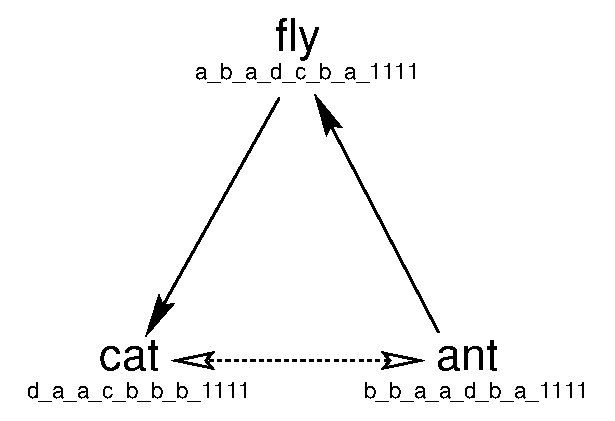
\epsfig{file=figures/antcatfly.eps}
\else
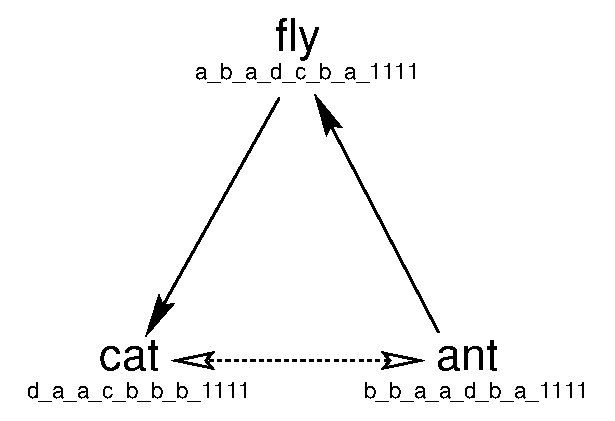
\psfig{file=figures/antcatfly.eps}
\fi
\caption{Echo agents initially present in experiments described in
this section.  Interactions among ants, caterpillars (``cat'') and
parasitic flies are coded by agent genotypes.  Open arrows indicate
mutualistic trade between ants and caterpillars.  Closed arrows
indicate direction of an attack in combat (flies attack caterpillars;
ants attack flies).  The genotype of each agent is indicated with 
loci in the following order: offense tag, defense tag, mating tag,
combat condition, trading condition, mating condition, trading resource,
and uptake mask.
\label{fig:antcatfly}}
\end{center}
\end{figure}

We have run experiments with a variety of initial conditions.  The two
most common setups are as follows: (1) start with a single founding
agent that is one mutation away from trading, fighting, and mating with 
itself, and (2) start with a small set of hand-designed agent types
that encode some interaction pattern of interest.  The experiments
reported here all use the second setup, consisting of three agent
types that form a trophic triangle.  However, we get similar results
when the first style of initial condition is used (data not shown).

Figure~\ref{fig:antcatfly} illustrates the initial conditions
used in the experiment detailed in this section.  This ant,
caterpillar, fly interaction network was described by Holland
\cite{Holland9?} [and is based on observations by Holldobler and
Wilson \cite{HolldoblerAndWilson90}].  The caterpillars secrete a
nectar which is collected by the ants.  In exchange, ants nurture
the caterpillars.  Parasitic flies attempt to consume caterpillar
larvae, while the ants defend their symbionts.  Initially, each site
in a world has ten agents of each genotype present, with ten letters
of each resource type in reserve.  No mating occurs initially, though
mutation could produce such an interaction during simulation.

% this paragraph used to be first in this subsection but PTH moved
% it here
The parameters used in our experiment are shown in
Table~\ref{tab:simulation-parameters}.  We vary the area
by defining worlds with multiple identical sites.  Agents
which fail to acquire resources during a time step are allowed to
migrate to one of the site's four neighbors to the north, south, east
or west.  Periodic boundary conditions are imposed on worlds
comprised of 1, 4, 16 or 64 sites.  Thus, agents live in toroidal
worlds of a fixed size; this is roughly analagous to living on an 
island of given area.  Independent simulations were run for both 1,000
and 10,000 iterations.

\begin{table}[t!]
\begin{center}
\begin{tabular}{|l|c|} \hline
Parameter & Value \\ \hline
Number of Resources & 4 \\
Trading Fraction & 0.5 \\
Interaction Fraction & 0.02 \\
Self Replication Fraction & 0.5\\
Self Replication Threshold & 2\\
Taxation Probability & 0.1 \\ \hline
Mutation Rate & 0.02 \\
Crossover Probability & 0.07 \\
Random Death & 0.0001 \\
Initial Vector & 10 \\
Production Vector & 10 \\
Maximum Vector & 100 \\
Maintenance Vector & 1 \\ \hline
\end{tabular}
\end{center}
\caption{Parameters used for Echo experiments described in text.  See
Section~\protect\ref{echo-structure} for a detailed description of each
parameter.  World-level parameters are above the line; site-specific 
parameters are below.  Resource parameters are indicated as vectors.  
In our experiments these values are equal for all four resources.
\label{tab:simulation-parameters}}
\end{table}

\subsection{The Neutral Model}
\label{neutral-model}

Neutral models are used in biology to evaluate what mechanisms are
necessary to produce a phenomenon of interest
\cite{Caswell76,NiteckiAndHoffman87}.  Here we are interested whether
tags and conditions affect patterns of diversity in Echo populations.
Non-random mating, competition or predation, and direct or indirect
mutualisms are all believed to regulate species diversity in
ecological communities.  The question for both Echo and the real world
is whether such mechanisms are 
necessary to produce patterns such as the species-area scaling
relation.  The neutral model we implemented substitutes the tag-based
interactions described in Section~\ref{agent-agent} with random
interactions.  When two agents are chosen to interact, the decision of
whether they will fight, trade, or mate is based on random tosses of a
biased coin, rather than string-matching criteria.  This adjustment 
is analagous to an ecology in which species interact with one another
randomly.  Aside from this modification, all other bookkeeping (i.e.,
resource assimilation, self-replication, migration, taxation, and
random death) is performed identically in both models.

%[MERGE IN WITH THE PREVIOUS PARAGRAPH]
%The neutral version of Echo replaces tag-based interactions with
%random interactions (see section~\ref{neutral-model}).  Thus, the
%neutral model removes the effect of the genome on agent-agent
%interactions.  If both versions of Echo exhibit the same patterns seen
%in nature, then one of two conclusions can be drawn.  Either Echo is
%not a minimal model (that is, not all of its mechanisms are needed to
%produce the relevant behaviors), or explanations in the ecological
%literature have posited more complexity than necessary
%\cite{Caswell76,ConnorSimberloff79,NiteckiAndHoffman87} to account
%for observed patterns.  [PETER: I still don't understand this second
%point] 
% PTH says: If the Preston distribution results from random processes,
%           why infer that other process (e.g., competition,
%           mutualisms, etc.) are responsible for the pattern?
%           By parsimony, random processes alone are necessary to produce
%           the pattern.

\begin{table}[t!]
\begin{center}
\begin{tabular}{|c||c|c|c||c|} \hline
& {\sc Combat} & {\sc Trade} & {\sc Mating} & {\sc Total} \\
& $P_{combat}\cdot P_{escape}$ & $(1-P_{combat})\cdot P_{trade}$ & $(1-P_{combat})\cdot P_{mating}$ & $P_{int}$ \\ \hline 
Neutral model & $1/4 \cdot 1/2$ & $(1-1/4) \cdot 1/8$ & $(1-1/4) \cdot 1/8$ & $10/32$ \\ \hline
Original model & $1/m^n \cdot P_{escape}$ & $(1-P_{combat})(1/m^n)^2$ & $(1-P_{combat})(1/m^n)^2$ & $P_{int}$ \\ \hline
n=0 & $1/1 \cdot 1/2$ & $(1-1) (1/1)^2$ & $(1-1) (1/1)^2$ & $1/2$ \\
n=1 & $1/4 \cdot 1/2$ & $(1-1/4) (1/4)^2$ & $(1-1/4) (1/4)^2$ & $7/32$ \\
n=2 & $1/16 \cdot 1/2$ & $(1-1/16) (1/16)^2$ & $(1-1/16) (1/16)^2$ & $\approx 1/32$ \\ \hline

%Neutral model & $\frac{1}{4} \times \frac{1}{2}$ & $(1-\frac{1}{4}) \times \frac{1}{8}$ & $(1-\frac{1}{4}) \times \frac{1}{8}$ & $\frac{10}{32}$ \\ \hline
%Original model & $\frac{1}{m^n} \times P_{escape}$ & $(1-P_{combat})(\frac{1}{m^n})^2$ & $(1-P_{combat})(\frac{1}{m^n})^2$ & $P_{int}$ \\ \hline
%n=0 & $\frac{1}{1} \times \frac{1}{2}$ & $(1-1) \times (\frac{1}{1})^2$ & $(1-1) \times (\frac{1}{1})^2$ & $\frac{1}{2}$ \\
%n=1 & $\frac{1}{4} \times \frac{1}{2}$ & $(1-\frac{1}{4}) \times (\frac{1}{4})^2$ & $(1-\frac{1}{4}) \times (\frac{1}{4})^2$ & $\frac{7}{32}$ \\
%n=2 & $\frac{1}{16} \times \frac{1}{2}$ & $(1-\frac{1}{16}) \times (\frac{1}{16})^2$ & $(1-\frac{1}{16}) \times (\frac{1}{16})^2$ & $\approx \frac{1}{32}$ \\ \hline
\end{tabular}
\end{center}
\caption{Comparison of probability values for interactions between
agents in neutral and original models.  The alphabet
size ($m$) for genotypes is the number of resources used (4 for our
simulations).  For the original model, probabilities are shown for
conditions of length ($n$) 0, 1 and 2.
\label{tab:neut-model-params}}
\end{table}

Parameters for the neutral model were chosen to produce the same
interaction probability between two randomly selected agents 
as in the original Echo model.  The chance an interaction will
occur between two randomly chosen agents is the sum of the
probabilities that combat, trade, or mating will occur
(Table~\ref{tab:neut-model-params}).  For the neutral 
model, probabilities of combat, trade, and mating were set at $1/4$,
$1/8$, and $1/8$, respectively.

As we described earlier, if an agent is attacked by another agent in
combat, the attacked agent is given a chance to flee from the
attacker.  The probability of escape equals the probability of losing
in combat.  In the neutral model, an agent will escape attack with a
probability of $1/2$.  In the neutral model, the chance of
being attacked and defeated is the product of the probability of
combat and the chance of escape ($1/4 \cdot 1/2 = 1/8$).  Thus, the
 probability that any interaction will occur between two selected 
agents in the neutral model is $10/32$.

%In the original model, the probability of escape varies with scores from 
%matching alleles in offense and defense tags in the combat matrix.
%The combat matrix used in our experiments assigns equal scores to
%matches at all loci, so the probability of escape from combat for any
%two agents with loci of the same length will be $1/2$.
In the original model, the probability any interaction will occur is
based on the chance of randomly matching a condition as a prefix of a
tag.  For mating and trade to happen, combat must not occur,
and each agent must match its condition as a prefix of the other's tag.
Denoting $n$ as the mean length of the conditions in agents' genomes,
we calculate the probability of any interaction occurring between two
agents in Echo to be $P_{int} = 1/2$ for $n=0$, $7/32$
for $n=1$, and $\approx 1/32$ for $n=2$.  For our experiment,
the mean length of conditions in the original model was 0.98, and
lengths of conditions for individual genotypes ranged from 0 to 6
(data not shown).  We conclude that the average interaction
probability is equal in the neutral and original versions of Echo.

\subsection{Experimental Design and Data Analysis}
\label{data-analysis}

Our experiments were designed to test whether or not $S_{tot} = cA^z$
in both the original and neutral versions of Echo.  To test this,
%whether $S \sim A^{1/4}$, 
we used a $4 \times 2 \times 2$ factorial
design, with $20$ replicates for each combination of world area (1, 4,
16, or 64 sites), number of iterations ($10^3$ or $10^4$ iterations),
and model type (original or neutral model).  For each replicate
population, we recorded $S_{tot}$ (number of species), $N_{tot}$
(number of individuals), and $N_{max}/N_{tot}$ (an index of dominance,
the fraction of the population represented by the most abundant species
\cite{Pielou77}).  We also calculated the mean number of species and
individuals per site ($S/$site and $N/$site).
Although other definitions of species in Echo have been considered
(see \cite{ForrestAndJones94}), in this study, a species is defined as
a unique genotype.  
%To test for significant treatment effects, we used two-way analysis
%of variance (ANOVA) \cite{Lindman74,Potvin93} 
%on three response variables: mean $S$ and $N$ per site, and dominance.
%Separate analyses were conducted for runs lasting $10^3$ and $10^4$
%iterations.  
% For a
% given set of treatment factors (the statistical ``model''), ANOVA
% breaks down variance into within treatment and between treatment
% components, then calculates a test statistic ($F$) from the ratio of
% between group error (``model'' sum of squares) to within group error
% (error sum of squares).  If this test value corresponds to a
% probability of 95\% or greater significance, we conclude the model
% accounts for more variation than by chance.  We tested models for all
% treatment factors (model type, area, and time) and their interactions.
% ANOVA was perfomed in SAS \cite{SAS85}.
% {\it Post hoc} comparisons were made for the area factor, to distinguish
% which areas exhibited different responses.  The {\it post hoc}
% comparisons were made with a Bonferroni correction to the significance
% test.  The Bonferroni correction controls experimentwise type I error
% rate, and is a conservative test for differences among treatment
% levels \cite{Philippi93}.

We used multiple regression to compare coefficients of species-area
functions in the original and neutral models.  
%Regression calculations were performed in SAS on the
%log$_2$-transformed species counts, and used backwards elimination to
%build the best regression equation.  Backwards elimination is an
%iterative procedure which fits a regression to all variables, then
%successively eliminates variables which do not contribute to the
%regression equation.  
The full regression equation was in the form
$\widehat{S_{tot}} = (\beta _1 + \beta _2)A^{(\beta _3 + \beta _4)} +
\epsilon$ for the original model and $\widehat{S_{tot}} = \beta _1
A^{\beta _{3}} + \epsilon$ for the neutral model.  A variable was
eliminated from our regression equation if it had less than 90\%
probability of being significantly different from 0.  To
interpret these regression equations, note that eliminating $\beta _4$
from the best regression equation implies that model type has no
significant effect on $z$, but that $\beta _3$ can be used to predict
$z$ for both models.  Similarly, eliminating $\beta _2$ implies that
model type has no significant effect on $c$, and can be predicted by
$\beta _1$ alone.  The $\epsilon$ term describes residual error.
Separate equations were built for runs of $10^3$ and $10^4$ iterations.

\subsection{Results}

% Preston curves
% this figure came from
% algodones:/landscape/users/phraber/projects/modeling-paper/preston-plots.  
% data were generated with the script sfi:~pth/projects/Echo/bin/preston
% for the following runs:
% model   time    area    seed            outfile
% orig    3       1       519477386       preston-a
% orig    4       64      237813364       preston-b
% neut    3       1       179905860       preston-c
% neut    4       64      87600382        preston-d
\begin{figure}[t!]
\begin{center}
\leavevmode
\ifepsf
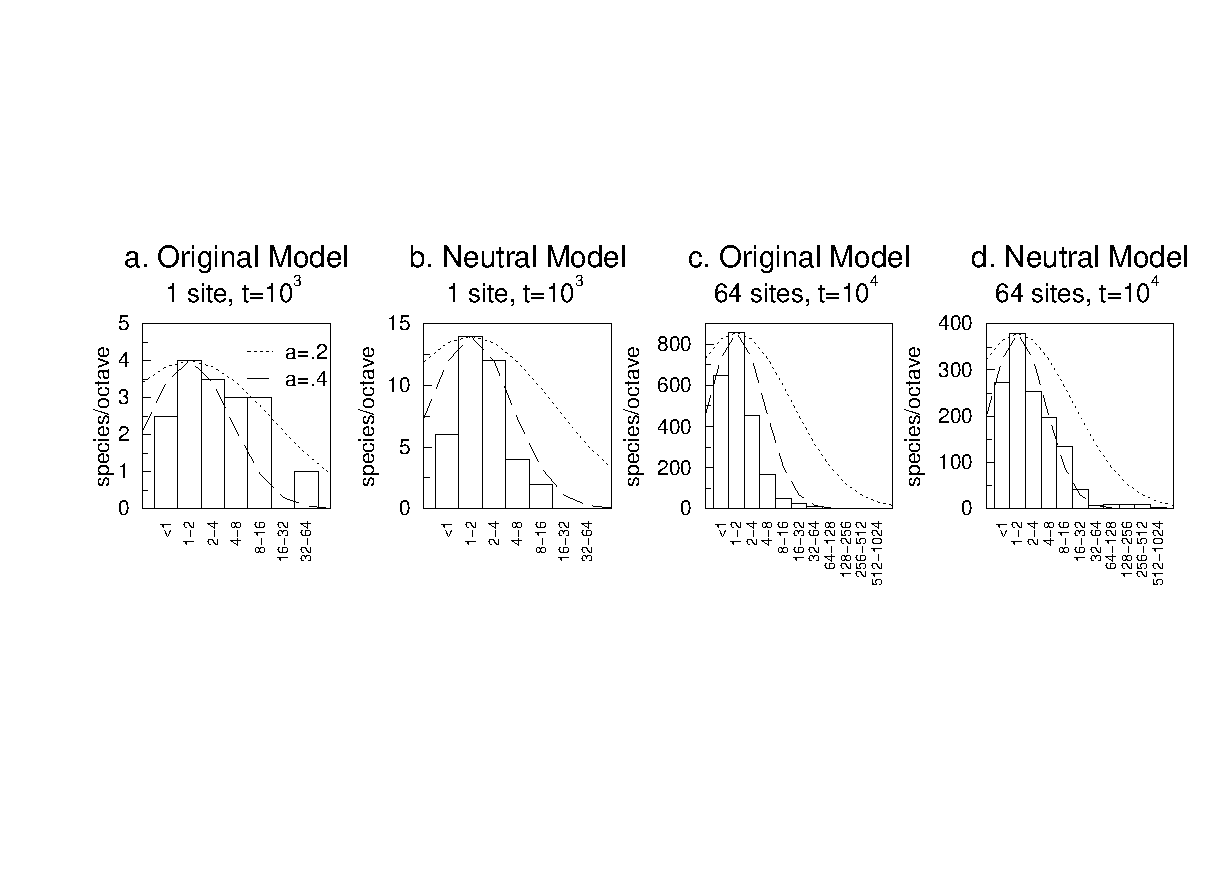
\epsfig{file=figures/preston-curves-h.ps,height=1.5in,width=6in,bbllx=0,bblly=140,bburx=620,bbury=350}
\else
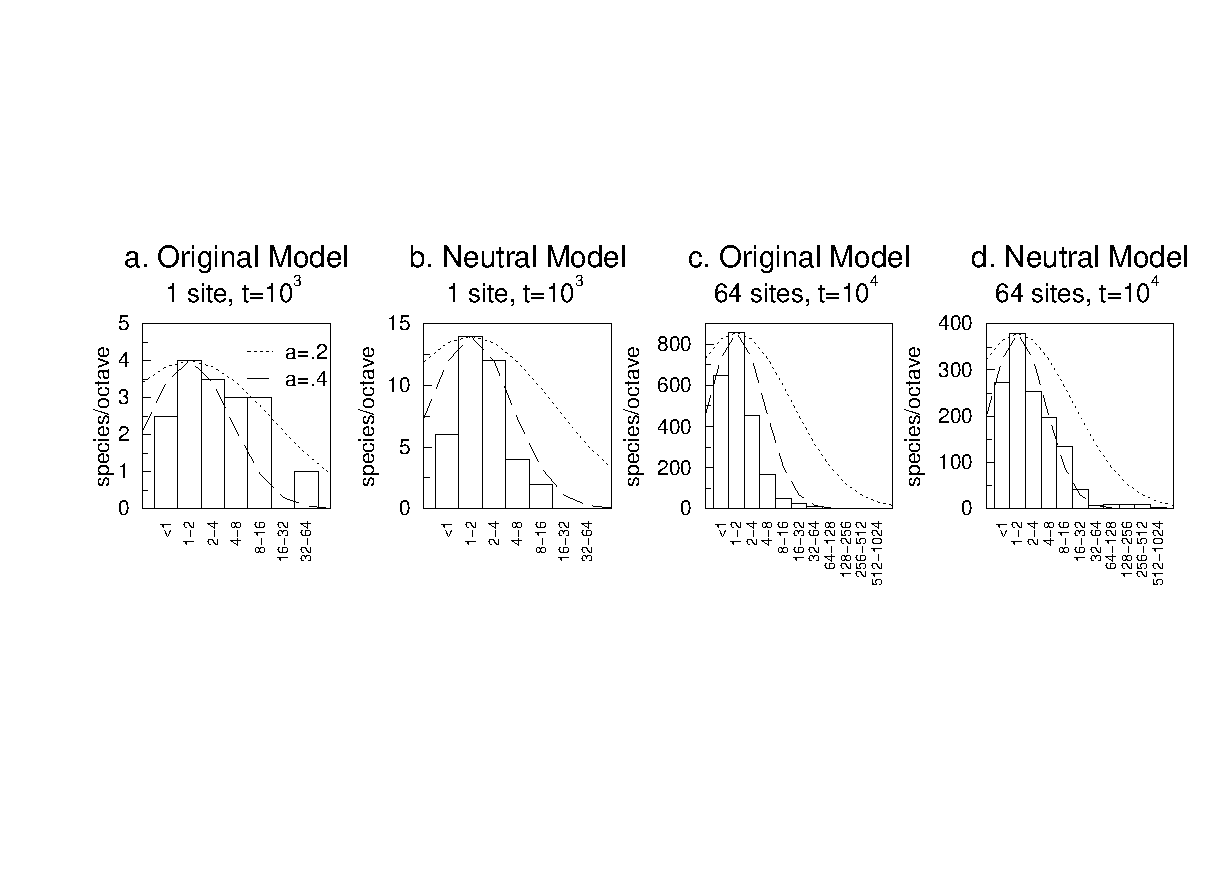
\psfig{file=figures/preston-curves-h.ps,height=2in,width=6in}
\fi
\caption{Preston curves from four Echo populations.  See
  section~\protect\ref{preston-distribution} for a description of
  Preston curves.  Populations are from original (a, c) and neutral
  (b, d) models, either for a one-site world at 1000 iterations
  (a, b), or for a 64-site world at 10,000 iterations (c, d).  Each
  population was randomly chosen from 20 replicates.  Expected values
  under Preston's canonical hypothesis are plotted as dotted and
  broken lines, for $a=.2$ and $a=.4$, respectively.
\label{fig:preston-curves}}
\end{center}
\end{figure}

Preston curves from typical populations are shown in
Figure~\ref{fig:preston-curves}, and additional data are reported in
\cite{ForrestAndJones94}.  Populations from both the original and
neutral model are plotted, for short runs in small worlds, and for
longer runs in larger worlds.  Distributions expected under Preston's
canonical hypothesis are plotted for comparison.  These data suggest
the pattern of genome abundances in Echo populations qualitatively
resembles Preston's log-normal distribution, although there are some
differences.  We have observed this general pattern in a wide variety
of Echo runs under a wide variety of different parameter settings and
initial conditions.  As we discussed earlier, we do not believe that a
careful quantitative comparison is possible, so the remainder
of our experiment focusses on the species-area scaling relation.

% ANOVA response variables (bar plots)
% this figure came from algodones:/landscape/users/phraber/projects/modeling-paper/sas/anova/means/histo.ps
\begin{figure}[t!]
\begin{center}
\leavevmode
\ifepsf
\epsfig{file=figures/anova-response-vars-h.ps,height=2.5in,width=6in,bbllx=80,bblly=330,bburx=730,bbury=780}
\else
%\psfig{file=figures/anova-response-vars-h.ps,height=2.5in,width=6in,bbllx=80,bblly=330,bburx=730,bbury=780}
\psfig{file=figures/anova-response-vars-h.ps,height=2.5in,width=6in}
\fi
\caption{Response variables from simulations of $10^3$ iterations
  (a, b, c) and $10^4$ iterations (d, e, f).  Species richness per site
  (a, d), population size per site (b, e) and dominance (c, f) are
  plotted as a function of area.  Solid (black) bars are from the
  original model and unfilled (white) bars are from the neutral model.
  Each bar represents a mean from twenty replicates.  Error bars
  indicate one standard deviation.
\label{fig:anova-response-vars}}
\end{center}
\end{figure}

In simulations lasting $10^3$ iterations, the neutral model
has more species per site than the original model.
(Figure~\ref{fig:anova-response-vars}a, b, c).  Increasing area
decreases number of species per site in the neutral model and
decreases dominance in the original model.  Number of individuals per
site is not affected by model type or area of the world.  

Variances in all response variables are greater in longer runs than
in shorter runs (Figure~\ref{fig:anova-response-vars}d, e, f).
Dominance and number of species per site do not differ with model type,
but the neutral model has more individuals per site than the
original model.  Increasing area increases the number of individuals per
site, and decreases dominance and number of species per site.

%[PETER: please explain someplace what you mean by dominance.-done]
%In the test for a species-area scaling relation, the analysis of
%variance on simulations lasting $10^3$ iterations indicates that the
%original and neutral versions of Echo have significantly different
%means for number of species per site and number of individuals per
%site (Table~\ref{tab:anova-results-t3},
%Figure~\ref{fig:anova-response-vars}a, b).  Dominance does not differ
%with model type (Table~\ref{tab:anova-results-t3},
%Figure~\ref{fig:anova-response-vars}c).  Increasing area has
%significant effects on mean species per site and dominance, but not on
%the number of individuals per site.  Treatment interaction effects
%[PETER: what does ``treament interaction effects'' mean?] are detected
%for species per site and dominance (Table~\ref{tab:anova-results-t3}).
%For runs lasting $10^4$ iterations, variances in response variables
%are greater (Figure~\ref{fig:anova-response-vars}d, e, f).  Model type
%has a significant effect on $N$/site only
%(Table~\ref{tab:anova-results-t4},
%Figure~\ref{fig:anova-response-vars}e).  
%Varying area has significant effects on all three response variables
%(Table~\ref{tab:anova-results-t4},
%Figure~\ref{fig:anova-response-vars}d, e, f).  
%Effects of a model type by area interaction have a marginally
%significant effect on $S$/site (Table~\ref{tab:anova-results-t4}).
%[PETER: need a little more prose here explaining all this.]
%[STEPH: let's combine these two tables, make them more compact, and
%do them in the same style as the other tables]
% ANOVA tables
% these data come from algodones:/algodones/users/phraber/projects/modeling-paper/sas/anova/anova-t3-not-log-xformed.lst
%\begin{table}[btp!]
%\caption{ANOVA results from simulations lasting $10^3$ iterations.
%Treatments are model type
%(original or neutral model) and world area (1, 4, 16 or 64 sites).
%Response variables are mean number of species per site, mean number of
%individuals per site, and dominance.  Asterisks indicate significance
%of the $F$ test ($P$).  [PETER: explain all headings---I couldn't understand
%this table.]
%% Tables:
%% ANOVA tables
%\label{tab:anova-results-t3}}
%\begin{center}
%\begin{tabular}{lrrrl} \hline \hline
%{\sc Source} & df & ss (I) & $F$ & \\ \hline
%\multicolumn{5}{c}{{\sc Mean S per site}} \\
%{\sc Type}                &   1 &  3107.6 &  294.66 & **** \\
%{\sc Area}                &   3 &  2489.4 &   78.68 & **** \\
%{\sc Type$\times$Area}    &   3 &   672.2 &   21.25 & **** \\
%{\sc Error}               & 152 &  1603.1 & & \\ \hline
%\multicolumn{5}{c}{{\sc Mean N per site}} \\
%{\sc Type}                &   1 &  125.8  &  15.59 & **** \\
%{\sc Area}                &   3 &   11.7  &   .48 & \\
%{\sc Type$\times$Area}    &   3 &   37.0  &   1.53 & \\
%{\sc Error}               & 152 & 1226.9  & & \\ \hline
%\multicolumn{5}{c}{{\sc Dominance}} \\
%{\sc Type}                &   1 & .0092 &    5.21 & \\
%{\sc Area}                &   3 & .3099 &   58.67 & **** \\
%{\sc Type$\times$Area}    &   3 & .1969 &   37.29 & **** \\
%{\sc Error}               & 152 & .2676 & & \\ \hline
%** $P \le .01$, *** $P \le .001$, **** $P \le .0001$.
%\end{tabular}
%\end{center}
%\end{table}
%% these data come from algodones:/algodones/users/phraber/projects/modeling-paper/sas/anova/anova-t4-not-log-xformed.lst
%\begin{table}[btp!]
%\caption{ANOVA results from simulations lasting $10^4$ iterations.
%  Treatments and response variables are as in
%  Table~\protect\ref{tab:anova-results-t3}
%\label{tab:anova-results-t4}}
%\begin{center}
%\begin{tabular}{lrrrl} \hline \hline
%{\sc Source} & df & ss (I) & $F$ & \\ \hline
%\multicolumn{5}{c}{{\sc Mean S per site}} \\
%{\sc Type} & 1 & 10.1 & 0.05 & \\
%{\sc Area} & 3 & 9305.8 & 15.28 & **** \\
%{\sc Type$\times$Area} & 3 & 3192.7 & 5.24 & ** \\
%{\sc Error} & 152 & 30863.1 & & \\ \hline 
%\multicolumn{5}{c}{{\sc Mean N per site}} \\
%{\sc Type} & 1 & 52531.9 & 31.24 & **** \\
%{\sc Area} & 3 & 87099.5 & 17.27 & **** \\
%{\sc Type$\times$Area} & 3 & 15089.7 & 2.99 & \\
%{\sc Error} & 152 & 255562.6 & & \\ \hline
%\multicolumn{5}{c}{{\sc Dominance}} \\
%{\sc Type} & 1 & 0.0177 & 2.16 & \\
%{\sc Area} & 3 & 0.4259 & 17.31 & **** \\
%{\sc Type$\times$Area} & 3 & 0.0164 & 0.66 & \\
%{\sc Error} & 152 & 1.2468 & & \\ \hline
%** $P \le .01$, *** $P \le .001$, **** $P \le .0001$.
%\end{tabular}
%\end{center}
%\end{table}
% END ANOVA tables

%regression coefficients
% these data come from algodones:/algodones/users/phraber/projects/modeling-paper/sas/SA/SvA-full.lst
\begin{table}[btp!]
\caption{Coefficients from multiple regression analysis.  Treatments
  of different durations ($T$) were analyzed separately.  Parameter
  estimates are shown for the best regression equation, after backwards
  elimination of parameters with $P>0.10$.  See
  section~\protect\ref{data-analysis} for a description of the multiple
  regression equations.  All parameters are
  significant at $P\le .001$.
\label{tab:regress-coeffs}}
\begin{center}
\begin{tabular}{|c|c||cc|cc||c|} \hline
\emph{T} & \emph{n} & $\beta _1$ & $\beta _2$ & $\beta _3$ & $\beta _4$ & $r^2$ \\
 & & \multicolumn{2}{c|}{($c$)} & \multicolumn{2}{c||}{($z$)} & \\ \hline \hline
$10^3$ & 160 & 5.39 & -.62 & .87 & .08 & .995 \\
$10^4$ & 160 & 5.78 & -.62 & .70 & .23 & .877 \\ \hline
\end{tabular}
\end{center}
\end{table}

A scaling relation
describes the species-area function in both models at $10^3$
iterations, and in the original model at $10^4$ iterations
(Figure~\ref{fig:species-area-curves}).  Mild curvilinearity might
be present in the species-area function for the neutral model at
$10^4$ iterations.  With this minor exception, we note that both
models demonstrate the hypothesized scaling relation.  Multiple
regression analyses indicate all terms in the full regressions
equation are statistically significant
(Table~\ref{tab:regress-coeffs}).  That is, we reject with more than
99\% confidence the null hypotheses that $\beta _2 = 0$ and $\beta _4
= 0$.  Thus, values of $c$ and $z$ for the original and neutral models
differ significantly.  Actual values for $z$ at $10^3$ iterations are
$0.95$ and $0.87$ for the original and neutral models, respectively 
(Figure~\ref{fig:species-area-curves}a).
Simulations of $10^4$ iterations yield $z$ values of $0.93$ and $0.70$ 
for original and neutral models (Figure~\ref{fig:species-area-curves}b).  

%SA curves
% this figure came from algodones:/landscape/users/phraber/projects/modeling-paper/sas/SA/SA.ps
\begin{figure}[t!]
\begin{center}
\leavevmode
\ifepsf
\epsfig{file=figures/species-area-curves-h.ps,height=3in,width=6in,bbllx=80,bblly=350,bburx=740,bbury=840}
\else
%\psfig{file=figures/species-area-curves-h.ps,height=3in,width=6in,bbllx=80,bblly=350,bburx=740,bbury=840}
\psfig{file=figures/species-area-curves-h.ps,height=3in,width=6in}
\fi
\caption{Species-area curves for $10^3$ (a) and $10^4$ iterations
  (b).  Species counts for the original model ($\bullet$) and
  neutral model ($\circ$) are plotted against area of the world.  Note
  that both axes are log$_2$-transformed.  Lines are regression fits
  using parameters in Table~\protect\ref{tab:regress-coeffs}.  Slope
  of each regression line ($z$) is indicated in the legend.  Each
  point is a mean of 20 replicates.  Error bars indicate one standard
  deviation.
\label{fig:species-area-curves}}
\end{center}
\end{figure}
            % \newpage ??
\section{Discussion}

Our results show that the original and neutral versions of Echo behave
differently with respect to species richness and population size
in a site, as well as the scaling exponent in the species-area 
relation.  This suggests that the dynamics of the two models differ.
%However, it is not clear which is a better model of ecological and
%evolutionary dynamics.  
Both models produce distributions of abundance which resemble Preston
distributions, though neither produces a canonical distribution.
Both models yield scaling exponents far greater than the expected
value of $\frac{1}{4}$.  We attribute this result to a combination of factors,
discussed below, some of which have interesting implications for the
Echo model.

Our choice of simulation parameters was largely arbitrary.
A different choice of parameter settings could yield different results
than observed here, and some combination of parameters might produce
the expected value.  However, our experience with Echo has shown that
the general patterns reported here appear to be relatively insensitive to
parameter settings.  We have obtained similar results in experiments
with lower mutation rates, increased interaction fractions, and
different initial populations (data not shown).

A second factor affecting our results is the definition of
species in Echo.  In this study, we used the provisional definition
of unique genotypes as species.  A previous study
\cite{ForrestAndJones94} defined species based on 
clustering genomes by a distance metric (number of mutations to
produce one genotype from another).  This clustering technique
produces curves that more closely approximate the canonical Preston
distribution.  Using that method here might reduce the number of
species in a population, and thus lower the slope of the
species-area curve.  We decided not to use the clustering technique
here because of the problem of defining species by an arbitrary
genetic distance, but it could significantly change the outcome of our
experiment by reducing the number of singletons.

Species-area curves are typically constructed by sampling from the
total number of individuals present, rather than a complete census.
We checked to see if sampling might affect our results by constructing
species-area curves using subsampling.  Rather than including each
individual in a sample with a probability of one, we tried
subsampling both $\frac{1}{10}$ and $\frac{1}{4}$ of the population and
recalculating the species-area curves.  This procedure did not
noticably change the slope of the curve (data not shown).  Sampling
and complete censusing of Echo populations produce similar
species-area curves.

In nature, habitat heterogeneity plays a role in limiting the
distributions of species across the landscape.  No species is so well
adapted as to be equally successful in all habitats.  This mechanism
to limit species success does not exist in the Echo worlds we have
studied to date.  Our Echo worlds are not heterogenous but are made
of similar sites tiled together.  In these simulations, there are no
gradients in resource availability or favorability of climate such as
those that are believed to limit organisms in nature.  Rather, a
species which is successful at one site in the world should be equally
successful throughout the world.  [SO, WHY DON'T WE DO SOME RUNS TO
TEST THIS?]

It is likely that the discrepancy between expected and observed values
for $z$ reflects an imbalance between rates of speciation and
extinction in our model.  New species are formed by mutating
existing species, and by recombining genotypes through mating.
Formation of new species is thus controlled by mutation and
recombination rates.  Species go extinct on the death of the last
surviving individual, whether through competition or by chance.
However, the mechanisms of extinction in natural systems may include
exogenous events never before experienced by the species.

Raup proposes that many extinctions could be caused by events that
occur on a time scale greater than species' evolutionary time scales
\cite{Raup91}.  This idea is promising, because it parsimoniously
explains how widespread species might suffer extinction.  If the
exogenous events were to occur on an evolutionary time scale, natural
selection should favor species that can tolerate such adversity.
Species with small populations are more likely to suffer extinction by
mechanisms such as fluctuations in population size or competition than
widespread species.  Again, this would have the effect of decreasing the 
slope of the species-area curve.  For a firmly established (widespread) 
species to suffer extinction requires some extreme circumstances, or rare
events.  Raup calls such unnatural events ``first strikes'' and argues
that these rare events play a major role in driving common species
to extinction.  Unlike earth, the Echo model we used here is a closed
system; there are no meteorite impacts or global changes in climate or
sea level to drive species nearer to extinction through previously
unencountered adversity.

We conclude from these considerations that the mechanisms in the
current implementation of Echo are not sufficient to limit species'
success.  Competition and random death as means for extinction are
insufficient to produce the quantity of extinctions necessary to agree
with empirically based predictions made by the species-area scaling
relation.  However, Echo does exhibit a robust species-area scaling
relation as well as a log-normal species-abundance curve similar to a
Preston curve.  The degree of quantitative agreement between these
curves and those found in natural ecosystems may be less important
than the fact that we see similar kinds of curves.
[PTH disagrees with this very stongly.  The whole point of the canonical
lognormal distribution is that a special kind of curve is observed.
Random processes can produce lognormal distributions, so it's easy to 
make curves which look like these.  The whole reason for using the neutral 
model is to ask whether these curves result from community interactions or 
noise.  PTH cares about degree of quantitative agreement between these
curves and those found in natural ecosystems.]

More generally, these results represent a first step towards
validating Echo as a model of natural ecological systems.  Echo is
clearly quite a different kind of model than those typically used in
ecological studies, and it is relevant to ask what we can hope to
learn from a highly abstract model that by design does not directly
correspond to any real system.  There are at least three possible
answers to such a question:
\begin{itemize}
\item Echo as a patch of dirt,
\item Echo as a flight simulator, and [STEPH: if we take John's name
off the paper we should either cite this or change the language slightly.]
\item Echo as a theory of complex adaptive systems.
\end{itemize}

By ``Echo as a patch of dirt,'' we mean to suggest the possibility of
constructing Echo worlds that do correspond directly to some real
ecosystem.  This would allow careful quantitative validation of Echo's
behavior and might possibly lead to concrete predictions.  This kind
of modeling is well beyond the current state of the Echo research
program.  Although it would be an important achievement for Echo to
simulate one real ecosystem accurately, this may not be its most
important contribution.  Other modeling systems have traditionally
focused on exactly this problem of making quantitative predictions
about the behavior of specific systems with given parameter settings.

A second use of Echo is as a kind of ``flight simulator'' to be used
for building intuitions about how ecosystems work, what is critical
to their stability, etc.  Under this view, Echo itself is a rich enough
ecology to be worth studying in its own right, along the lines that we
have outlined in the previous sections.
We can study patterns of behavior,
e.g., how resources flow through different kinds of ecologies, how
cooperation among agents can arise through evolution, and arms races
\cite{Holland94}.  We can also use such a model to identify 
parameters or collections of parameters that are critical, i.e., to
perform a kind of sensitivity analysis.  As with any simulation tool, 
it is much easier to run hypothetical what-if experiments than to conduct
experiments on a real system.  If a model like Echo were successful
and correct, it would enable users to build deep intuitions about how
different aspects of an ecological system affect one another,
important dependencies, and an appreciation of how evolution interacts
with the internal dynamics of an ecosystem.  The neutral model that we
introduced in this paper is an example of how these intuitions can be
developed and explored.  This is perhaps the most important
contribution that models like Echo can make.
%[MAYBE A MORE CONCRETE STATEMENT HERE ABOUT PETER'S AMERICAN NATURALIST PAPER HERE.]

A third, and more ambitious, view of Echo is as a theory of complex
adaptive systems \cite{Holland95a}.  Echo can be viewed as a
computational artifact that captures what we believe are the essential
components and interactions in a wide variety of CAS.  As such, it
encodes a theory about which mechanisms are relevant and which are
not.  The theory can be confirmed or disconfirmed by running the model
under a wide variety of operating conditions and observing the extent
to which the expected macro-level behaviors arise spontaneously.  Our
experiments on species diversity are an example of such a confirmation
process, and our introduction of the neutral model provides another
way of testing the extent to which the current Echo mechanisms are all
required to produce the behaviors of interest.  It should be noted
that the version of Echo reported here is an early attempt at a broad
CAS theory, and we expect that many of the details will need to be
modified over time (e.g., to address the problem of extinctions) and
when careful comparisons to other CAS (e.g., economic models) are made
Nevertheless, an important contribution of computational systems like
Echo is to distill features that are common across many CAS in a
testable model.

Although we are optimistic about the insights that artificial-life
models like Echo can contribute to understanding real ecosystems and
other CAS, it is important to note that such models have several
apparent drawbacks.  These include a mapping problem, what concrete
questions they can address, scaling issues, and nonlinear interactions
(already discussed).  We discuss the first three of these issues
briefly in the following paragraphs.

Because CAS models tend to strip away many details, it is often
impossible to say what any component of one of these models
corresponds to in the real world---a mapping problem.  In
the immune system, for example, many theoretical immunologists use string
matching to model receptor/ligand binding
\cite{PerelsonAndOster79}.  Patterns of bits (or other symbols) are
used to represent both molecular shape and electrostatic charge.
Consequently, it is difficult to say what one bit in the model
corresponds to in the immune system.  Because different alphabets and
different matching rules can have very different properties, the
challenge is to select an alphabet and matching rule that have general
properties similar to the real system without worrying too much what
each bit really stands for \cite{Smith94a}.  By contrast, most
theories of modeling are based on the premise that a correspondence
can be established between the modeled system and the primitive
components of its model.

As a consequence of this mapping problem, it is not always clear what
scientific questions are being addressed by CAS models.  In more
conventional simulation-based modeling, models are used to make
quantitative predictions based on certain predicated inputs, for
example, to determine optimal parameter values.  Agent-based models of
CAS are rarely able to make this kind of quantitative prediction, and
as a result the focus is on identifying broad categories of behavior
and critical parameters (but not necessarily the exact critical
parameter values), as we discussed earlier.

A third problem faced by agent-based models is one of scale.  Because
they are simulations, agent-based models typically operate on vastly
different time scales of evolution and with much smaller population
sizes than those of the systems they model.  Also, we tend to be
intolerant of high failure rates such as those often observed in
nature.  For example, consider the selection algorithms typically used
in genetic algorithms.  Selection pressure is maintained at an
artificially high rate and often scaled to maintain increased pressure
near the end of a run.  Evolution thus occurs orders of magnitude more
quickly than in natural systems, and as a result, we may lose some of
the richness of the natural evolutionary process.

Despite these drawbacks, we believe that there is much to be learned
from discrete, agent-based models such as Echo.  [REITERATE the 
discrete/spatial inhomogenetity stuff from intro].
\input{conclusions}
\section{Acknowledgments}

This work was supported by the Santa Fe Institute (Project 2050) and
ONR grant N00014-95-1-1000.  Hraber was supported by NSF grant
BSR-9107339 awarded to B.T. Milne.  Support for Forrest was provided
by NSF grant IRI-9157644 and ONR grant N00014-95-1-0364.  Acknowledge
THAW foundation??  John Holland conceived of and designed the original
Echo model on which our work is based, and he suggested many of the
ideas in this paper.  James Brown, Marc Feldman, Simon Fraser, Timothy
Keitt, Bruce Milne, and Erik Schultes have all provided many useful
comments on Echo.  Brown suggested the examination of Preston's work
on species abundance. We also thank Josh Epstein, Rob Axtell and all
those involved in Project 2050 at the Santa Fe Institute, the
Brookings Institute and the World Resources Institute for their
comments.  Computational facilities were provided by the Santa Fe
Institute and the Sevilleta LTER.




\bibliographystyle{plain}
\bibliography{references}

\end{document}

% Local Variables:
% TeX-master:"main"
% End:
